\capitulo{4}{Técnicas y herramientas}

Esta parte de la memoria tiene como objetivo presentar las técnicas metodológicas y las herramientas de desarrollo que se han utilizado para llevar a cabo el proyecto. Se comentará de manera breve, las diferentes opciones y la razón porque estás fueron descartadas.

%%%%SISTEMAS OPERATIVOS
\section{Sistema Operativo}

\subsection{Opciones elegidas}

\subsubsection{Microsoft}
~\href{https://www.microsoft.com/es-es}{Microsoft} es el sistema operativo generalista por excelencia. Es de sobra conocido, con sus pros y contras. Fue elegido por comodidad, ya que es el que tengo instalado en mis ordenadores. Además el IDE usado~\pageref{visual} para el desarrollo, será de la misma compañía, por lo que hay mayor optimización para este sistema.

\subsubsection{Android}
~\href{https://www.android.com/intl/es_es/}{Andorid} es un sistema operativo móvil desarrollado por Google. Está basado en el kernel de Linux. Tiene casi toda la cuota de mercado de telefonía. Este se ha usado en mi \emph{smartphone} personal y en las máquinas virtuales, con el fin de probar las aplicaciones en dispositivo físicos y virtualiazdos respectivamente.

\subsection{Alternativas descartadas}

\subsubsection{Ubuntu}
~\href{https://ubuntu.com/}{Ubuntu} es un sistema operativo de código abierto, distribuido bajo una licencia libre. Está basado en Debian, distribución de Linux. Se desarta porque no iba a instalar otro sistema operativo en mis ordenadores personales.


\subsubsection{macOS X}
~\href{https://www.apple.com/es/macos}{macOs} sistema operativo creado por Apple, basado en Unix. Se descarta por que se quiere trabajar con dispositivos Android. Pero en el caso de que se quiera desarrollar para iOS~\pageref{ios}, es indispensable usarlo aquí, porque a la hora de compilar, tira de las librerías internas de este sistema operativo.

\subsubsection{iOS}~\label{ios}
~\href{https://www.apple.com/es/ios}{iOS} sistema operativo para \emph{smartphones} creado por Apple, basado en Unix. Se descarta por que se quiere trabajar con dispositivos Android. Pero en el caso de que se quiera desarrollar para iOS~\pageref{ios}, es indispensable usarlo aquí, porque a la hora de compilar tira de las librerías internas del sistema operativo.

%%CONTROL DE VERSIONES
\section{Control de versiones}

\subsection{Opciones elegidas}

\subsubsection{Git}
~\href{https://git-scm.com//}{Git} es un software de control de versiones, pensado para trabajar con gran cantidad de archivos, con el fin de llevar el registro de los cambios y coordinar a las personas que los comparten. Es gratuito y de código abierto.

Me he decantado por él, porque lo usé durante las prácticas curriculares y extracurriculares de forma intensa, mediante la herramienta Git Bash, ya que mediante comando me siento más cómodo que con una interfaz. Aunque también la dispone mediante el comando \emph{gitk}.

\subsubsection{GitHub}\label{github}
~\href{https://github.com/}{Github} es una plataforma web, recientemente comprada por Microsoft, usada para el control de versiones con las funciones de Git. Entre las diferentes herramientas a destacar: wiki para cada uno de los proyectos, gráficos, funcionalidades de red social, gestor de proyectos, entre otras.

Se escogió esta porque la hemos usado durante el grado y es de sobra conocida. Además ofrece la posibilidad de integración con la herramienta Zenhub~\pageref{zenhub}, para la gestión del proyecto, teniendo las dos cosas centralizadas en el mismo lugar, lo que facilita el proceso de desarrollo.

\subsection{Alternativas descartadas}

\subsubsection{Gitlab}
~\href{https://gitlab.com/}{Gitlab}es igual que Github pero de código abierto ya que tiene licencia MIT. También lo usé en la empresa durante las prácticas pero fue descartado porque me parece de menor calidad. En cuanto a espacio este tiene 10 GB a favor, en contra del 1 GB de Github.

\subsubsection{Bitbucket}
~\href{https://bitbucket.org/product//}{Bitbucket} es otra web más para el control de versiones. Esta enfocado más a la empresa privada, ya que se suele integrar muy bien con otras herramientas de gestión de proyectos. Se descarto por el poco uso que he tenido con este.

\subsubsection{Extensiones Visual Studio Code}
Hay una gran cantidad de herramientas para el control de versiones en la tienda de este editor de código, puede ser práctico, pero las interfaces pueden ser liosas. Por eso me gusta más mediante comando, descartando rápidamente esta opción.

%%% GESTION DE PROYECTOS
\section{Gestión de proyecto}

\subsection{Opción elegida}

\subsubsection{Zenhub}\label{zenhub}
~\href{https://bitbucket.org/product//}{Zenhub} es una herramienta de gestión de proyectos, que viene por defecto integrada en Github~\pageref{github}, lo que implica a usarla sin pensarlo mucho. En mi caso lo que más usé fue el tablero de \emph{kanban} donde poder ver las \emph{issues} que me planificaba para cada \emph{sprint}. Ofrece diferentes tipos de gráficos, el que mejor se encajaba a la planificación fue de \emph{burndown}, ya que me permite ver lo ideal del proyecto y la progresión que llevo. No me gustó que las tareas las cierra por días en vez de por horas.

\begin{figure}[h]
	\centering
	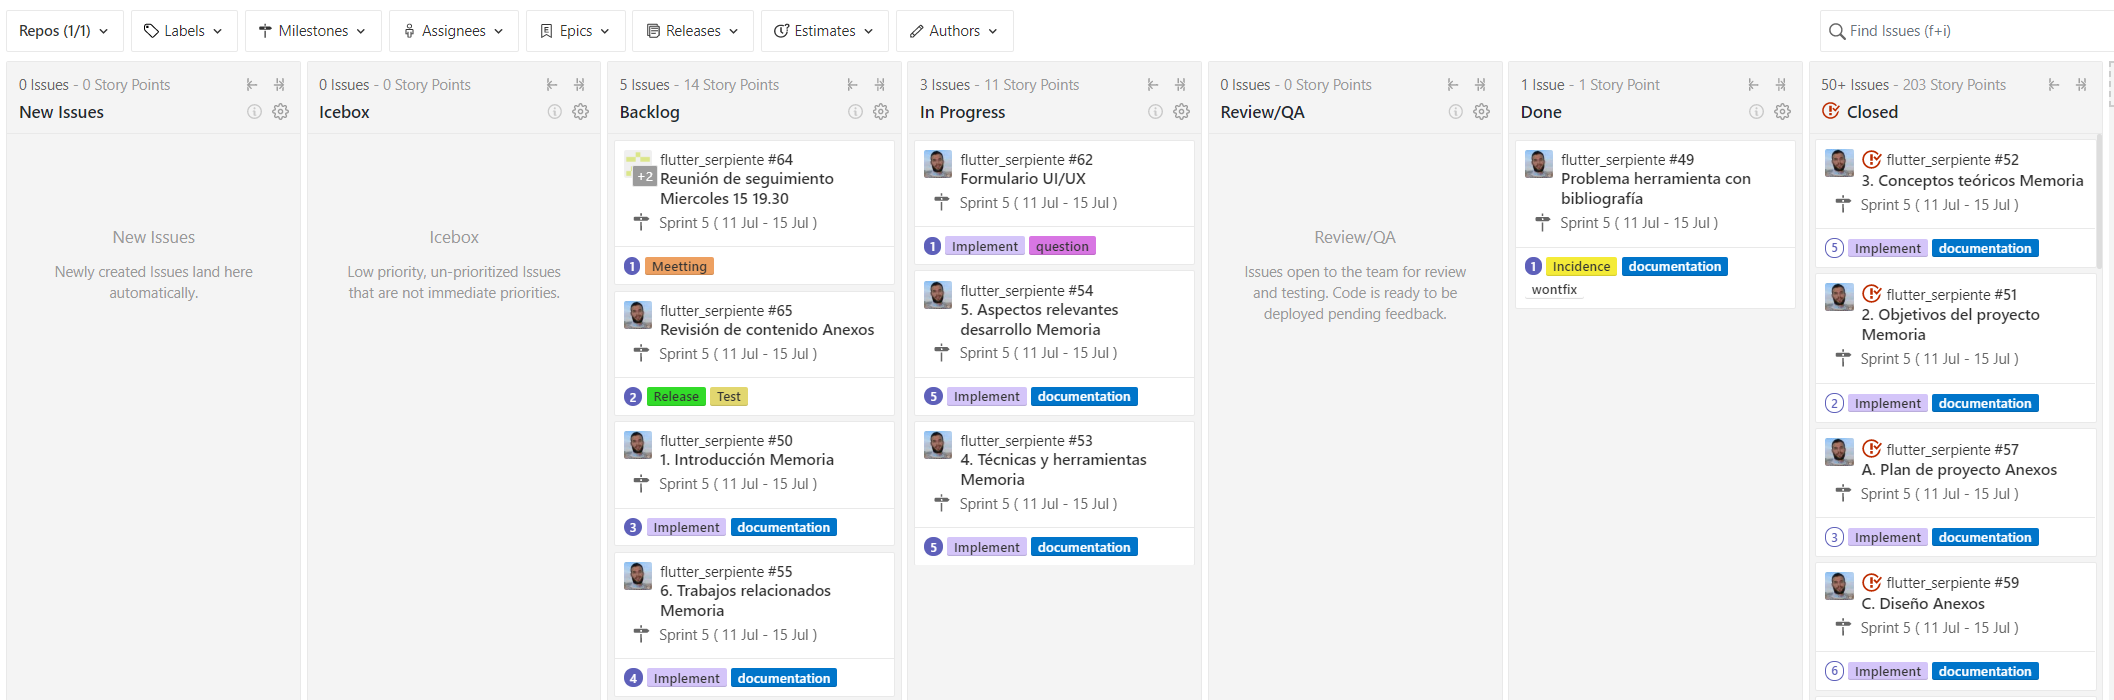
\includegraphics[width=1\textwidth]{teoria/kanban.png}
	\caption{Herramienta Zenhub}\label{fig:zenhub}
\end{figure}

\subsection{Alternativas descartadas}

\subsubsection{Jira}
~\href{https://www.atlassian.com/es/software/jira}{Jira} es una herramienta web propietaria, para el control, seguimiento de errores e incidencias, dentro de la gestión de proyectos. La conozco porque la usé durante las prácticas curriculares, me gustaba mucho, pero no me parece cómoda para lo que quería hacer. Ya que esta herramienta esta orientada en la mejora de procesos en la empresa, que al desarrollo de software.

\subsubsection{Trello}
~\href{https://trello.com/es}{Trello} es una herramienta de gestión de proyectos, con interfaz móvil y web. Usa el sistema kanban como Zenhub~\pageref{zenhub} y tiene integración con Github~\pageref{github}, pero me parece que no encaja en proyectos unipersonales, como era mi caso. Ya que el enfoque es más colaborativo, con grandes grupos de trabajo, donde es necesario compartir documentos con los requisitos, etc ...

%%% ENTORNOS DE PROGRAMACION
\section{Entorno de desarrollo integrado (IDE)}

\subsection{Opción elegida}

\subsubsection{Visual Studio Code}~\label{visual}
~\href{https://code.visualstudio.com/}{Visual Studio Code} es un editor de código fuente desarrollado por Microsoft, cuya licencia es MIT. Esta es totalmente gratuita, con una cantidad enorme de extensiones o \emph{pluggins}, que minimizan esfuerzos, además de la integración con git, que permite ver los cambios en tiempo real. 

Esta facilidad de uso hicieron que me decantase por él.

\subsection{Alternativas descartadas}

\subsubsection{Android Studio}\label{androidstudio}
~\href{https://developer.android.com/studio}{Android Studio} es la herramienta oficial de desarrollo de aplicaciones móviles para el sistema operativo Android. La licencia es Apache 2.0. y sustituye a Eclipse~\pageref{eclipse} como el entorno de desarrollo preferido por Google.

Este IDE se descarta para la creación de código, pero no para las máquinas virtuales.

\subsubsection{Eclipse}~\label{eclipse}
~\href{https://www.eclipse.org/}{Eclipse} es la plataforma software compuesta de varias herramientas de programación de código abierto. Se descartó por ser un IDE no recomendado por parte de Google. Además que a mi parecer es algo tosco.

%% MV
\section{Entorno de virtualización}

\subsection{Opción elegida}

\subsubsection{Android Studio}
~\href{https://developer.android.com/studio}{Android Studio}~\pageref{androidstudio} fue elegido para el despliegue de la aplicación en las máquinas virtuales que ofrece este IDE. Es eficiente y simple, centrado en Android. La creación de las VM es muy cómoda, ya que tiene todo integrado, (con cuatro clicks de ratón se puede lanzar una).

Sumado a que algunas herramientas de Visual Studio Code tiran de estas máquinas, hace que sea la opción más recomendable.

\subsection{Alternativas descartadas}

\subsubsection{Virtual Box}
~\href{https://www.virtualbox.org/}{Virtual Box} es un software de virtualización desarrollado por Oracle. Es de sobra conocido, ya que lo hemos usado durante el grado. Puede desplegar Android, pero al no estar integrado en el desarrollo de aplicaciones, se descató.


%% HERRAMIENTAS DE COMUNICACIÓN
\section{Herramientas de comunicación}

\subsection{Opciones elegidas}

\subsubsection{MS Teams}
~\href{https://www.microsoft.com/es-ww/microsoft-365/microsoft-teams/download-app}{Teams} es la herramienta de comunicación y colaboración integrado en el paquete ofimático de \emph{Office} de Microsoft. Se usó esta herramienta porque con la cuenta de la universidad tenemos acceso a ella y mis tutores de proyecto fueron quienes me la propusieron.

\subsubsection{Outlook}
~\href{https://www.microsoft.com/es-es/microsoft-365/outlook/email-and-calendar-software-microsoft-outlook}{Outlook} es una herramienta de Microsoft para la gestión de la información personal, integrado en la \emph{suite} de Microsoft Office. Se ha usado porque la cuenta de la universidad esta integrada con la plataforma.

\subsection{Alternativas descartadas}

\subsubsection{Gmail}
Es un servicio de correo electrónico proporcionado pro Google. Se descarta porque no tiene integración con la plataforma de la universidad de Burgos.

%% Herramientas para latex
\section{Documentación}

\subsection{Opciones elegidas}

\subsubsection{TexStudio}
~\href{https://www.texstudio.org/}{TexStudio} es un editor de Latex de código abierto, licencia GNU, muy similar a texmaker~\pageref{textmaker}, ya que es un \emph{fork} de este. Lo que hizo decantarme por el fue la corrección ortográfica interactiva y resaltado de la sintaxis.

\subsubsection{Zotero}
~\href{https://www.zotero.org/}{Zotero} es un gestor de referencias bibliográficas, cuya licencia es AGPL, siendo gratuito. Tiene una extensión para el navegador que ayuda mucho.

\subsection{Alternativas descartadas}

\subsubsection{TexMaker}\label{textmaker}
~\href{https://www.xm1math.net/texmaker/}{Texmaker} es un IDE gratuito para escribir documentos en Latex, su licencia es GPL.

\subsubsection{Overleaf}
~\href{https://www.overleaf.com/}{Overleaf} herramienta web para la edición de documentos escritos en Latex. Esta opción fue descartada porque al ser web, no me permite llevar un seguimiento del versionado como lo puedo hacer, si lo tengo en local con git.

\subsubsection{MS Word}
Editor de documentos de Microsoft, muy conocido, dentro del paquete de ofimática. Se descartó porque la universidad ofrece una plantilla en Latex, de gran calidad y que este no permite el control de versiones.

%% Herramientas varias Google chrome
\section{Herramientas}

\subsection{Opción elegida}

\subsubsection{Google Chrome}
Es un navegador web de código cerrado desarrollado por Google, siendo gratuito. Se ha usado este sin plantear alternativas, porque lo llevo usando desde hace muchos años. Fue usado como 'navaja suiza', ya que es una herramienta de herramientas, que ha sido usado para multitud de cosas, como:

\begin{itemize}
	\item Para descargar programas, paquetes, librerías...
	\item Para la búsqueda de información.
	\item Edición de imágenes.
	\item Generador de iconos \href{https://romannurik.github.io/AndroidAssetStudio}{romannurik}
	\item Creación de diagramas \href{https://app.creately.com}{creately}
	\item Armonía de color \href{https://color.adobe.com/es/create/color-wheel}{Adobe color}
\end{itemize}

%%%METODOLOGIAS
\section{Metodologías}

\subsection{Scrum}
Marco de trabajo para el desarrollo ágil de software, implementando una estrategia iterativa incremental, con revisiones y reuniones con los tutores de proyecto cada 5 días.

\subsection{Desarrollo en cascada}
Es un desarrollo en secuencia, es decir, una vez se pasa de etapa, no se puede volver atrás, se divide en \emph{steps} muy diferenciados, que se adapta my bien con las metodologías ágiles. 

\begin{figure}[h]
	\centering
	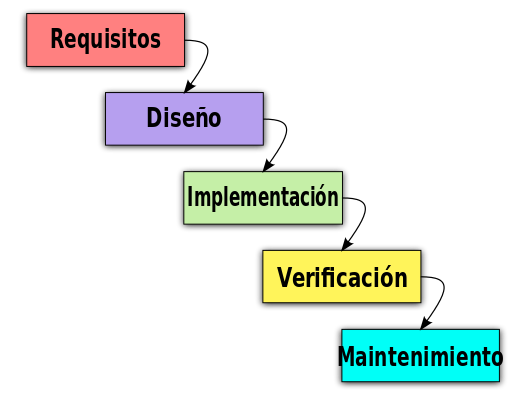
\includegraphics[width=0.8\textwidth]{teoria/cascada.png}
	\caption{Desarrollo en cascada}\label{fig:cascada}
\end{figure}

\subsection{Bolígrafo y cuaderno}
Para mi la parte más importante de toda la gestión del proyecto, reuniones, diseño de las interfaces, control de las horas, planificación, caja negra ... 

Siempre lo he tenido a mi lado como soporte, como se puede ver ~\ref{fig:soporte}:

\begin{figure}[h]
	\centering
	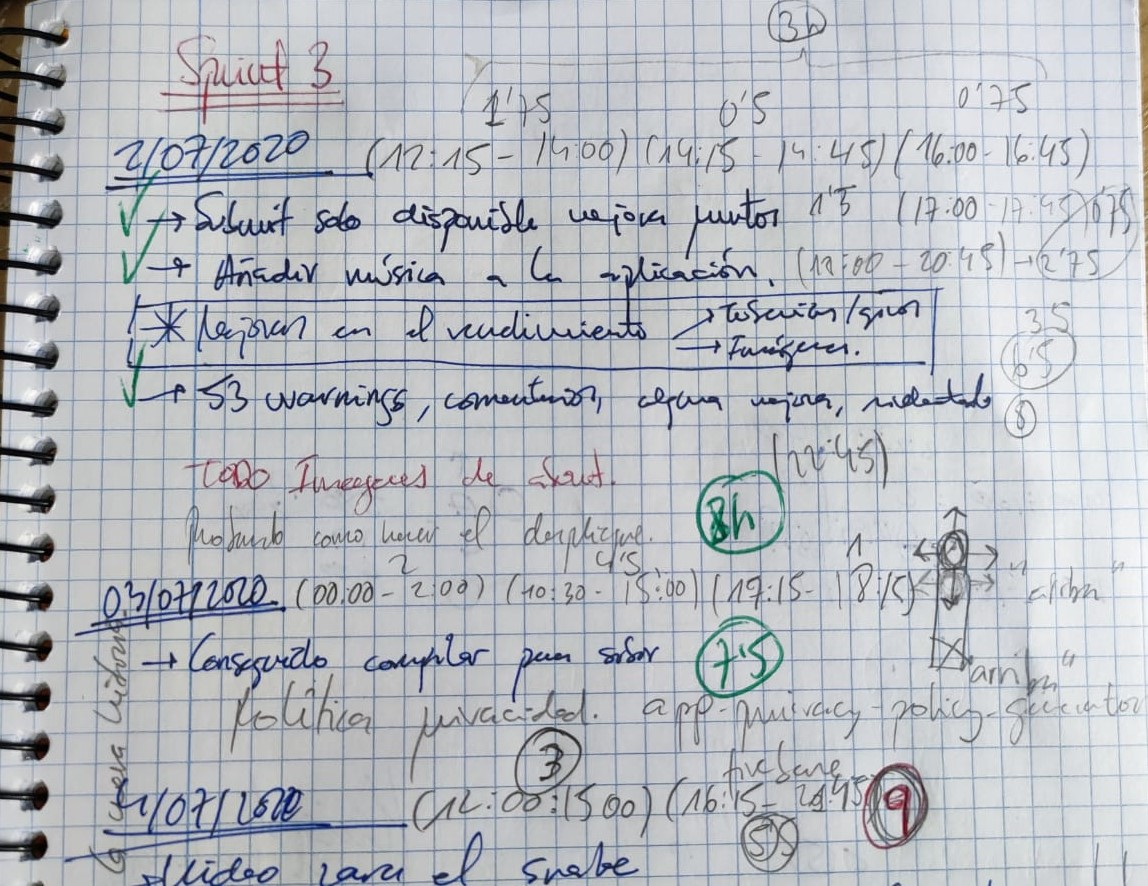
\includegraphics[width=1 \textwidth]{teoria/soporte.jpeg}
	\caption{Cuaderno}\label{fig:soporte}
\end{figure}

\section{Bibliotecas}

\subsection{Material Design}
Es una normativa de diseño o guía de estilos para garantizar una homogeneidad en la visualización dentro de Android. Está desarrollada por Google.

\subsection{Firebase}
Plataforma para el desarrollo de aplicaciones móviles, creada por Google en el 2014. Dispone de una gran cantidad de herramientas de mucha calidad.

\subsection{Play Services }
Librería que permite usar a terceros todas las herramientas ofrecidas por Google.




